\documentclass[oneside,14pt]{extarticle}
\usepackage[utf8]{inputenc}
\usepackage[english,ukrainian]{babel}
\usepackage{amssymb,amsfonts,amsmath,amsthm,mathtext,textcomp}

\usepackage[includehead, headsep=0pt, footskip=0pt, top=2cm, bottom=2cm, left=2cm, right=1cm]{geometry}
\usepackage{indentfirst}
\usepackage[onehalfspacing]{setspace}
\usepackage[headings]{fancyhdr}
\usepackage{etoolbox}
\usepackage{flafter}
\usepackage{listings}
\usepackage{graphicx}
\usepackage{float}
\usepackage[labelsep=period]{caption}
\lstset{
	breaklines=false
}
\usepackage{array}
\fancyhf{}
\renewcommand{\headrulewidth}{0pt}
\pagestyle{fancy}
\fancyfoot[R]{\thepage}
\lstset{breaklines=true,}
\graphicspath{ {./pictures} }

\lstset{
	language=c,
	tabsize=4,
	keepspaces,
	showstringspaces=false,
}
\graphicspath{ {./pictures} }
\setlength{\parindent}{4em}
\setlength\tabcolsep{5px}

\newcommand\subject{Моделювання та аналіз програмного забезпечення}
\newcommand\lecturer{доцент кафедри ПЗ \\ Сердюк П.В.}
\newcommand\teacher{викладач кафедри ПЗ \\ Микуляк А.В.}
\newcommand\mygroup{ПЗ-22}
\newcommand\lab{5}
\newcommand\theme{Поведінкові шаблони проектування}
\newcommand\purpose{Здобути навички використання поведінкових шаблонів проектування при моделюванні програмних систем}

\begin{document}
\begin{normalsize}
	\begin{titlepage}
		\thispagestyle{empty}
		\begin{center}
			\textbf{МІНІСТЕРСТВО ОСВІТИ І НАУКИ УКРАЇНИ\\
				НАЦІОНАЛЬНИЙ УНІВЕРСИТЕТ "ЛЬВІВСЬКА ПОЛІТЕХНІКА"}
		\end{center}
		\begin{flushright}
			\textbf{ІКНІ}\\
			Кафедра \textbf{ПЗ}
		\end{flushright}
		\vspace{70pt}
		\begin{center}
			\textbf{ЗВІТ}\\
			\vspace{10pt}
			до лабораторної роботи № \lab\\
			\textbf{на тему}: “\textit{\theme}”\\
			\textbf{з дисципліни}: “\subject”
		\end{center}
		\vspace{50pt}
		\begin{flushright}
			
			\textbf{Лектор}:\\
			\lecturer\\
			\vspace{10pt}
			\textbf{Виконав}:\\
			
			студент групи \mygroup\\
			Коваленко Д.М.\\
			\vspace{10pt}
			\textbf{Прийняв}:\\
			
			\teacher\\
			
			\vspace{28pt}
			«\rule{1cm}{0.15mm}» \rule{1.5cm}{0.15mm} 2023 р.\\
			$\sum$ = \rule{1cm}{0.15mm}……………\\
			
		\end{flushright}
		\vspace{\fill}
		\begin{center}
			\textbf{Львів — 2023}
		\end{center}
	\end{titlepage}
		
	\begin{description}
		\item[Тема.] \theme.
		\item[Мета.] \purpose.
	\end{description}

	\section*{Завдання}
Розробити структурні шаблони проектування відповідно до прецедентів обраного
варіанту ігрової логіки. Вибрати один з прецедентів, для якого найбільш доцільно
застосувати структурний шаблон (не всі прецеденти цього потребуватимуть).

	Представити діаграму класів ігрового проекту (із відображенням на ній використаних
	шаблонів).

	\section*{Хід виконання}
	
	\begin{figure}[H]
		\centering
		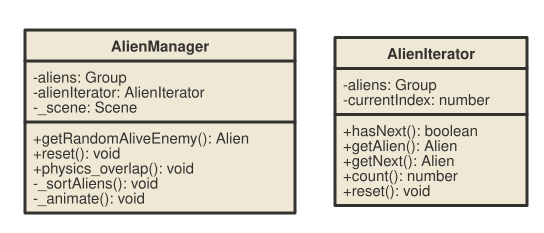
\includegraphics[]{iterator}
		\caption{UML діаграма реалізації шаблону Iterator}
	\end{figure}
	
	\begin{figure}[H]
		\centering
		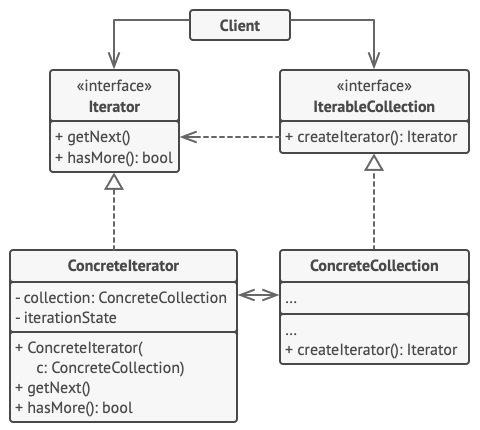
\includegraphics[]{iterator-ex}
		\caption{UML діаграма прикладу реалізації шаблону Iterator}
	\end{figure}
	
	\begin{small}
		\begin{lstlisting}

class AlienIterator {
	private aliens: Phaser.Physics.Arcade.Group;
	private currentIndex: number;
	
	constructor(group: Phaser.Physics.Arcade.Group) {
		this.aliens = group;
		this.currentIndex = 0;
	}
	
	hasNext(): boolean {
		return this.currentIndex < this.aliens.getLength();
	}
	
	getAlien(index: number): Alien {
		return this.aliens.getChildren()[index - 1] as Alien;
	}
	
	getNext(): Alien {
		this.currentIndex++;
		return this.aliens.getChildren()[this.currentIndex-1] as Alien;
	}
	
	count(): number {
		return this.aliens.getLength();
	}
	
	reset() {
		this.currentIndex = 0;
	}
}
		\end{lstlisting}
	\end{small}
	
	\begin{figure}[H]
		\centering
		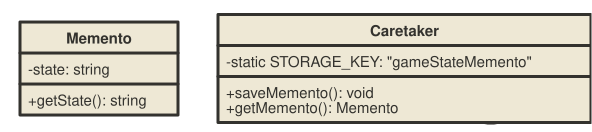
\includegraphics[width=\textwidth]{memento}
		\caption{UML діаграма реалізації шаблону Memento}
	\end{figure}
	
		\begin{figure}[H]
		\centering
		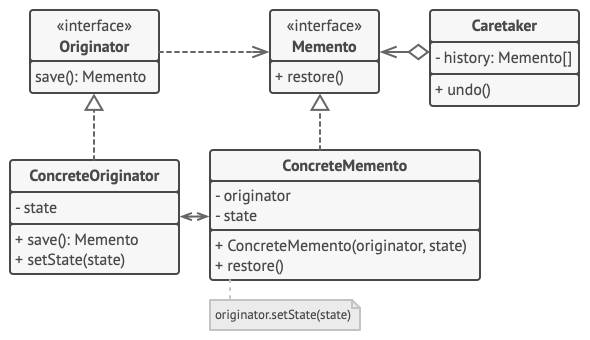
\includegraphics[width=\textwidth]{memento-ex}
		\caption{UML діаграма прикладу реалізації шаблону Memento}
	\end{figure}
	
	\begin{small}
		\begin{lstlisting}
		export class Memento {
			private state: string;
			
			constructor(state: string) {
				this.state = state;
			}
			
			public getState(): string {
				return this.state;
			}
		}
		
		export class Caretaker {
			private static readonly STORAGE_KEY = "gameStateMemento";
			
			public saveMemento(memento: Memento): void {
				localStorage.setItem(Caretaker.STORAGE_KEY, memento.getState());
			}
			
			public getMemento(): Memento | null {
				const state = localStorage.getItem(Caretaker.STORAGE_KEY);
				if (state) {
					return new Memento(state);
				}
				return null;
			}
		}
		\end{lstlisting}
	\end{small}
	
	\begin{figure}[H]
		\centering
		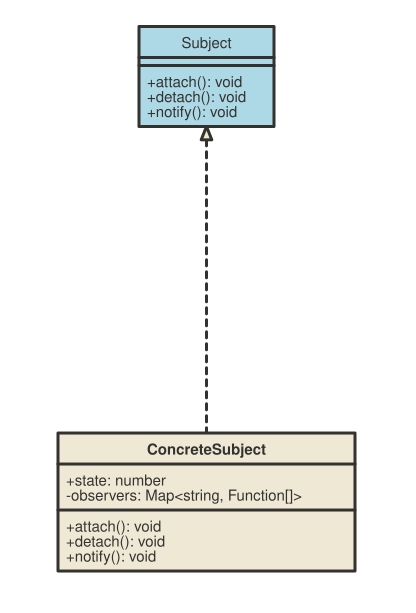
\includegraphics{observer}
		\caption{UML діаграма реалізації шаблону Observer}
	\end{figure}
	
		\begin{figure}[H]
		\centering
		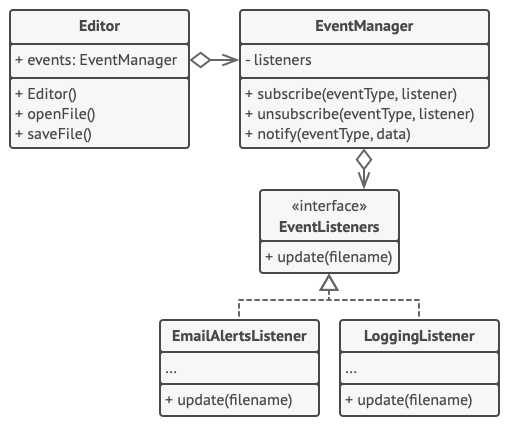
\includegraphics{observer-ex}
		\caption{UML діаграма прикладу реалізації шаблону Observer}
	\end{figure}
	
	\begin{small}
		\begin{lstlisting}
export interface Subject {
	attach(event: string, observer: Function): void;
	detach(event: string): void;
	notify(event: string): void;
}

export class ConcreteSubject implements Subject {
	public state: number;
	private observers: Map<string, Function[]> = new Map();
	
	public attach(event: string, observer: Function): void {
		this.observers.set(event, [...(this.observers.get(event) || []), observer]);
	}
	
	public detach(event: string): void {
		this.observers.delete(event);
	}
	
	public notify(event: string): void {
		this.observers.get(event).forEach((observer) => {
			observer();
		});
	}
}
		\end{lstlisting}
	\end{small}
	
	\section*{Висновки}
	   Під час виконання лабораторної роботи я здобув навички використання поведінкових шаблонів проектування при моделюванні програмних систем.
\end{normalsize}
\end{document}
